\chapter{Methodology}\label{ch:method}
This chapter describes the key idea, the proposed framework and methodology used in this thesis. A comparison between different image-to-image translation models using GANs is provided. Also, the architecture of text detection and text recognition models used for the OCR engine has been presented. This chapter discusses, in brief, each of the components used in the overall framework and their implementation procedures.
\newline

        The image-to-image translation is the class of computer vision problems where the goal is to learn the mapping between input and target domain. The applications of image-to-image translation range from style transfer, colorization, sketches to photo, and image super-resolution. In this thesis, we have investigated three different image-to-image translation GANs: Pix2pix, CycleGAN and FactorGAN to improve the readability of texts present in the steel type plate/nameplate images. Then the best generator model from the three GANs is selected and integrated with the pre-trained text detection \& text recognition model.

\section{Pix2pix GAN}
	\cite{isola2017image} proposed pix2pix (pixel to pixel) Generative Adversarial Network that has shown to produce realistic and detailed synthetic images. Pix2pix is a supervised image-to-image translation model that uses conditional GANs to learn a function to map input image to output image.  

\subsection{Architecture}
Similar to the standard GAN, the pix2pix model consists of two components i) Generator and ii) Discriminator as shown in Figure \ref{fig:pix}. The generator transforms the input image to an image in the target domain while the discriminator measures the similarity of the input image to image passed randomly either generated by generator or the real image and predicts the probability of the image being real. The pix2pix model is a type of conditional generative model with a target image as additional information. 

\begin{figure}[H]
\centering
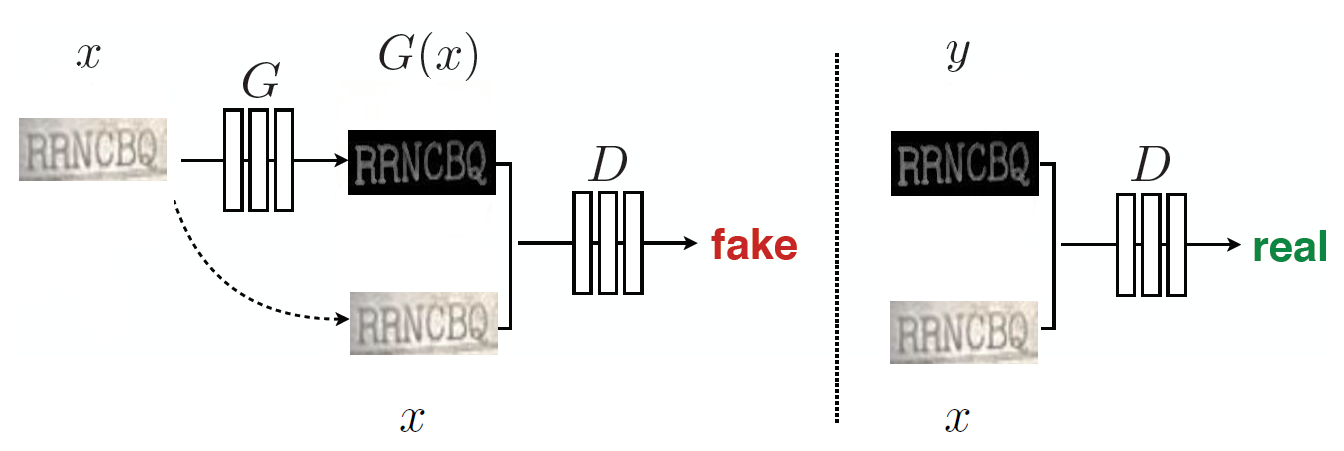
\includegraphics[width=5in]{images/pix2pix.png}
\caption[Architecture of pix2pix]{Architecture of pix2pix. Source: Adapted from \citep{isola2017image}}
\label{fig:pix}
\end{figure}

In contrast to the standard conditional GANs, the generator takes the source image with no noise as input whereas both the source image and target image are passed to the discriminator as shown in Figure \ref{fig:pix}. The generator is trained with adversarial loss and L1 loss to produce a meaningful translation of a source image to a target image. Also, the randomness is added to the network in the form of dropout. The architecture of the generator and the discriminator is explained in detail which is as follows:

\subsubsection*{Generator}

	For the generator architecture, the ResNet framework proposed by \citeauthor{he2016deep} was used. Residual Network (ResNet) is a CNN architecture consists of a series of residual blocks with skip connections to address the problem of vanishing gradients. The vanishing gradients problem occurs in deep neural networks when the weights of the initial layer not getting updated properly during back-propagation as the repeated multiplication makes the gradient small. Thus, the performance gets saturated with more layers in the network. Apart from this problem, they showed that adding more layers to the neural network slows down the training and does not improve accuracy. ResNet uses the identity matrix via skip connection that multiplies the gradient by 1 during backpropagation. Thus, it preserves the gradient and avoids information loss \citep{he2016deep,resnet}. 

\begin{figure}[H]
\centering
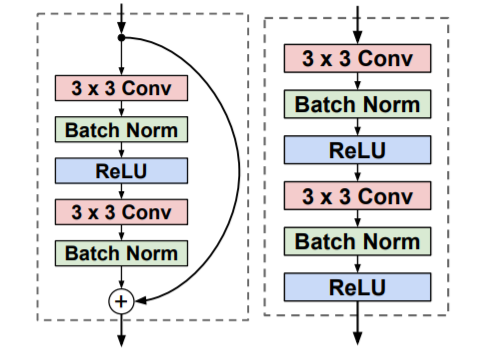
\includegraphics[width=4in]{images/resnetblock.PNG}
\caption[Difference between residual block (left) vs ordinary CNN (right) connections]{Difference between residual block (left) vs ordinary CNN (right) connections. Source: Supplementary material, \citep{johnson2016perceptual}}
\label{fig:resblock}
\end{figure}

The differentiating factor of ResNet from a CNN is their skip connection which is shown in Figure \ref{fig:resblock}. The skip connection adds the original input to the output of the convolution block. In traditional CNNs, each layer output is fed as input to the next layer, but with skip connections, each layer output is passed to consecutive layers as well as the non-consecutive layers. This helps in solving the problem of vanishing gradient and the identity matrix helps in maintaining the performance of initial layers with the higher layers \citep{resnet}. In our approach, the generator accepts an input image of size 600 x 400 x 3 and generates an output image of the 600 x 400 x 1. The full generator architecture is shown in Table \ref{tab:tab1}. \\

\begin{table}[h]
\centering
\begin{tabular}{|c|c|c|c|} 
\hline
\textbf{~ Block~} & \textbf{~ Filters} & \textbf{~Filter size~} & \textbf{~Stride}  \\ 
\hline
Conv-BN-ReLU      & 64                 & 7x7                    & 1                 \\ 
\hline
Conv-BN-ReLU      & 128                & 3x3                    & 2                 \\ 
\hline
Conv-BN-ReLU      & 256                & 3x3                    & 2                 \\ 
\hline
Residual Block1   & 256                & 3x3                    & 1                 \\ 
\hline
Residual Block2   & 256                & 3x3                    & 1                 \\ 
\hline
Residual Block3   & 256                & 3x3                    & 1                 \\ 
\hline
Residual Block4   & 256                & 3x3                    & 1                 \\ 
\hline
Residual Block5   & 256                & 3x3                    & 1                 \\ 
\hline
Residual Block6   & 256                & 3x3                    & 1                 \\ 
\hline
Residual Block7   & 256                & 3x3                    & 1                 \\ 
\hline
Residual Block8   & 256                & 3x3                    & 1                 \\ 
\hline
Residual Block9   & 256                & 3x3                    & 1                 \\ 
\hline
ConvT-BN-ReLU     & 128                & 3x3                    & 2                 \\ 
\hline
ConvT-BN-ReLU     & 64                 & 3x3                    & 2                 \\ 
\hline
Conv-tanh         & 1                  & 7x7                    & 1                 \\
\hline
\end{tabular}
\caption{Architecture of pix2pix generator}
\label{tab:tab1}
\end{table}
The generator consists of encoder, 9 ResNet blocks and decoder blocks. Each encoder and decoder block consists of a convolution layers, a batch normalization (BN) layer followed by the ReLU activation function. Each ResNet block has two connections from its input, one connection going through a series of convolutions, batch normalization \& activation functions and the other connection skipping over that series as shown in the Figure \ref{fig:resblock}.

\subsubsection*{Discriminator}

The PatchGAN architecture proposed by \cite{li2016precomputed} was used for the discriminator. It compares NxN patches of the image instead of the entire image to classify if it is real or fake. Thus, the PatchGAN is more suitable for producing sharp high-frequency detail and have shown great classification performance in GANs. We used the default 70 x 70 patches as suggested in the pix2pix paper. The discriminator architecture is shown in Table \ref{tab:tab2}. Here LReLU represents the Leaky ReLU activation function.

\begin{table}[H]
\centering
\begin{tabular}{|c|c|c|c|} 
\hline
\textbf{Block~}        & \textbf{Filters} & \textbf{Filter size~} & \textbf{Stride}  \\ 
\hline
Conv-LReLU~~           & 64               & 4x4                   & 2                \\ 
\hline
Block 2 Conv-BN-LReLU~ & 128              & 4x4                   & 2                \\ 
\hline
Block 3 Conv-BN-LReLU~ & 256              & 4x4                   & 2                \\ 
\hline
Block 4 Conv-BN-LReLU~ & 512              & 4x4                   & 1                \\ 
\hline
Block 5 Conv-Sigmoid~  & 1                & 4x4                   & 1                \\
\hline
\end{tabular}
\caption{Architecture of pix2pix discriminator}
\label{tab:tab2}
\end{table}

It consists of 5 blocks of convolution layers. The Leaky ReLU with 0.2 negative slope is used as an activation function. The first convolutional layer consists of 64 filters and it is upscaled after each block. At the final layer, a sigmoid activation function is used to predict if the 70 x 70 patch image is real or fake.

\subsection{Loss function}
The loss function of the pix2pix is the same as the conditional GAN as discussed in the earlier section. The $L_1$ loss is added extra to the loss function since the goal of the generator is to generate realistic images such that it fools the discriminator. The $L_1$ loss calculates the pixel-wise difference between the source image and the target image. Thus forcing the generator to produce images close to the ground truth. The adversarial loss \citep{isola2017image} is given by
\begin{equation*}
L\textsubscript{adv}(G,D)=\mathbb{E}_{x,y}[log D(x,y)] + \mathbb{E}_{x,z}[log(1-D(x,G(x,z))]
\end{equation*}
The $L_1$ loss \citep{isola2017image} is given  by 
\begin{equation*}
L\textsubscript{L1}(G)=\mathbb{E}_{x,y,z}[\lVert y - G(x,z) \rVert_1]
\end{equation*}
And the final objective function \citep{isola2017image} is the sum of the adversarial loss and the $L_1$ loss which is given  by

\begin{equation*}
G^*=arg\underset{G}{min}\underset{D}{max}L\textsubscript{adv}(G,D)\; + \;\lambda L\textsubscript{L1}(G)
\end{equation*}
\noindent
where $\lambda$ is the scalar used to determine the importance of the $L_1$ loss.

\section{CycleGAN}
CycleGAN is an unsupervised method for training image-to-image translation models. They learn the characteristics and styles from an image collection of the source domain and translates it to the target domain in the absence of paired data. \\
\begin{wrapfigure}{r}{0.6\textwidth}
\centering
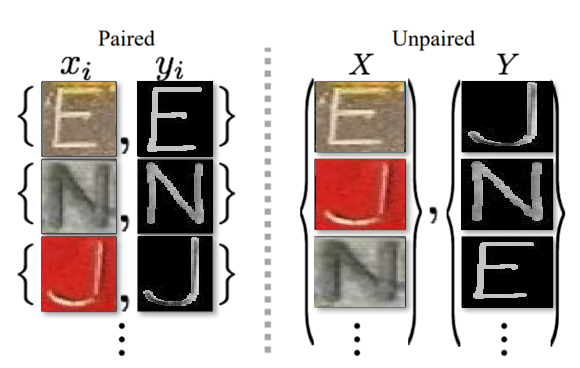
\includegraphics[width=0.5\textwidth]{images/newcyc.png}
\caption[Paired \& unpaired datasets]{Paired \& unpaired datasets. Source: Adapted from \citep{CycleGAN2017}}
\label{fig:pau}
\end{wrapfigure}
	The need for one to one mapping is eliminated by transforming the image from the source domain to the target domain and then back to the source domain just like translating a sentence from English to German and from German to English. 
\newline

	The authors conducted experiments on various image datasets such as horse $\leftrightarrow$ zebra, apple $\leftrightarrow$ orange, photo $\leftrightarrow$ monet, etc. Relaxing the one to one mapping makes the CycleGAN a more powerful method to tackle a variety of problems like the translation of noisy steel type plate images to clear images.

\subsection{Architecture}

Every image in a paired dataset is manually mapped from domain X to domain Y. Thus images in both domains share some common features. This pairing defines a meaningful relationship between images in both domains. In pix2pix, the generator takes input from domain X and translates it to an image close to domain Y. The CycleGAN with an unpaired dataset does not have this luxury since there is no meaningful transformation that it can learn.
The difference between the paired and unpaired dataset is shown in Figure \ref{fig:pau}. To establish a meaningful relationship in the unpaired dataset, \citeauthor{CycleGAN2017} introduced the concept of cycle consistency. The cycle consistency refers to the ability of translating an image from domain X to domain Y and then the generated image is translated back again to domain X. The architecture of CycleGAN is shown in Figure \ref{fig:cycarch}.

\begin{figure}[H]
\centering
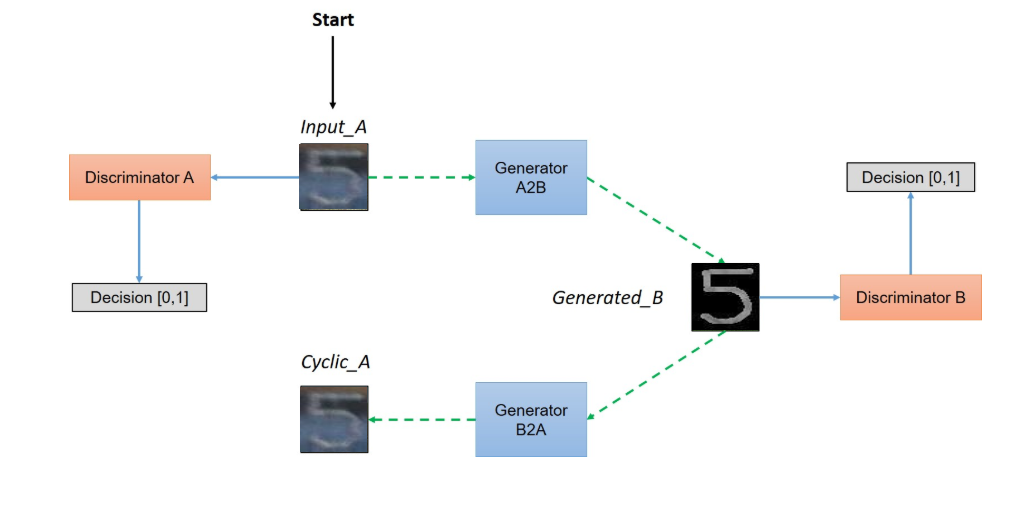
\includegraphics[width=5in]{images/cycGANarch.PNG}
\caption[Architecture of CycleGAN]{Architecture of CycleGAN. Source: Adapted from \citep{CycleGAN2017}}
\label{fig:cycarch}
\end{figure}

A generator will map the input image from a source domain to some image in the target domain with a constraint that the generated image must share some features that can map back to its original image. Thus the CycleGAN architecture consists of two generators G and F. The goal of generator G is to map X domain to Y domain such that G: X\textrightarrow Y and the other generator F will map Y domain to X such that F: Y\textrightarrow X. These generators have their respective discriminators $D_x$ and $D_y$. Discriminator $D_x$ forces generator G to translate images from domain X into an output that is indistinguishable from the images of domain Y and vice versa for Discriminator $D_y$.

\subsubsection*{Generator}
The same ResNet-9 blocks discussed in the pix2pix section was used as the architecture for both generators. Since the two generators are used, the images are resized to 300 x 300 to adapt to the memory requirements of the system. The instance normalization is replaced by batch normalization since multiple GPUs are used for training. The full generator architecture is explained in detail in Table \ref{tab:tab3}.

\begin{table}[H]
\centering
\begin{tabular}{|c|c|c|c|} 
\hline
\textbf{Block~} & \textbf{Filters} & \textbf{Filter size~} & \textbf{Stride}  \\ 
\hline
Conv-IN-ReLU    & 64               & 7x7                   & 1                \\ 
\hline
Conv-IN-ReLU    & 128              & 3x3                   & 2                \\ 
\hline
Conv-IN-ReLU    & 256              & 3x3                   & 2                \\ 
\hline
Residual Block1 & 256              & 3x3                   & 1                \\ 
\hline
Residual Block2 & 256              & 3x3                   & 1                \\ 
\hline
Residual Block3 & 256              & 3x3                   & 1                \\ 
\hline
Residual Block4 & 256              & 3x3                   & 1                \\ 
\hline
Residual Block5 & 256              & 3x3                   & 1                \\ 
\hline
Residual Block6 & 256              & 3x3                   & 1                \\ 
\hline
Residual Block7 & 256              & 3x3                   & 1                \\ 
\hline
Residual Block8 & 256              & 3x3                   & 1                \\ 
\hline
Residual Block9 & 256              & 3x3                   & 1                \\ 
\hline
ConvT-IN-ReLU   & 128              & 3x3                   & 2                \\ 
\hline
ConvT-IN-ReLU   & 64               & 3x3                   & 2                \\ 
\hline
Conv-tanh       & 1                & 7x7                   & 1                \\
\hline
\end{tabular}
\caption{Architecture of CycleGAN generator}
\label{tab:tab3}
\end{table}

\subsubsection*{Discriminator}
The PatchGAN discussed in the pix2pix section was used as the architecture for both the discriminators with the default setting 70 x 70. The full discriminator architecture is explained in detail in Table \ref{tab:tab4}.

\begin{table}[H]
\centering
\begin{tabular}{|c|c|c|c|} 
\hline
\textbf{Block~}        & \textbf{Filters} & \textbf{Filter size~} & \textbf{Stride}  \\ 
\hline
Conv-LReLU~~           & 64               & 4x4                   & 2                \\ 
\hline
Block 2 Conv-IN-LReLU~ & 128              & 4x4                   & 2                \\ 
\hline
Block 3 Conv-IN-LReLU~ & 256              & 4x4                   & 2                \\ 
\hline
Block 4 Conv-IN-LReLU~ & 512              & 4x4                   & 1                \\ 
\hline
Block 5 Conv-Sigmoid~  & 1                & 4x4                   & 1                \\
\hline
\end{tabular}
\caption{Architecture of CycleGAN discriminator}
\label{tab:tab4}
\end{table}

\subsection{Loss function}

	The loss function of CycleGAN needs to satisfy the following condition - i.e., the generated image should always be mapped back to its original image.
\newline

	Let the two generators be G, F and two discriminators $D_x$, $D_y$. The goal of the generators is to translate an image from domain X to Y and vice versa. Let the training samples in the domain X is defined as $\{x_i\}_{i=1}^N$ and training samples in the domain Y is defined as $\{y_j\}_{i=1}^M$. The distribution of the data is defined as the $x\sim p_{data}(x)$ and $y\sim p_{data}(y)$. The loss function of CycleGAN is defined by two losses: i) Adversarial loss and ii) Cycle consistency loss.
\newline

	The adversarial loss is used to match the distribution of generated images with the target domain. It is applied to both the generators. The adversarial loss \citep{CycleGAN2017} for generator G that translates the image from domain X to domain Y such that G: X\textrightarrow Y is given by
\begin{equation*}
L\textsubscript{GAN} (G,D_Y,X,Y)=\mathbb{E}_y\sim p_{data}(y)[log D_Y(y)] \; + \; \mathbb{E}_x\sim p_{data}(x)[log(1-D_Y(G(x))]
\end{equation*}
Likewise for generator F that translates the image from domain Y to domain X such that F: Y\textrightarrow X is given by,
\begin{equation*}
L\textsubscript{GAN}(F,D_X,Y,X)=\mathbb{E}_x\sim p_{data}(x)[log D_X(x)] \; + \; \mathbb{E}_y\sim p_{data}(y)[log(1-D_X(F(y))]
\end{equation*}

The cycle consistency loss enables both the generators to be stable and consistent. This loss regulates the GAN training process and makes sure that the generator does not generate any random permutation of images in the target domain \citep{CycleGAN2017}. It is given by

\begin{equation*}
L\textsubscript{cyc}(G,F)=\mathbb{E}_{x\sim p_{data}(x)}[\lVert F(G(x)) \; - \; x \rVert_1] \; + \; \mathbb{E}_{y\sim p_{data}(y)}[\lVert G(F(y)) - y \rVert_1]
\end{equation*}

Combining these two losses, 	
\begin{equation*}
L\textsubscript{GAN}\;(G,F,D_X,D_Y) = L\textsubscript{GAN}\;(G,D_Y,X,Y) \;+ \;L\textsubscript{GAN}\;(F,D_X,Y,X) \;+\; \lambda L\textsubscript{cyc}(G,F)
\end{equation*}
where $\lambda$ controls the importance of cycle consistency loss. So, the final objective function \citep{CycleGAN2017} is given by
\begin{equation*}
G^*,F^*=arg\underset{G,F}{min}\underset{D_X,D_Y}{max}L(G,F,D_X,D_Y)
\end{equation*}

\section{FactorGAN}
The last GAN that is investigated in this thesis is \cite{stoller2019training} proposed FactorGAN. Even though the GANs have been producing realistic images with greater success, they rely heavily on the amount of training data. Even though the datasets for the everyday objects are widely available, the datasets for specific industrial use case remains scarce. In the case of pix2pix, the generation of image pairs is time consuming, requires a lot of manual annotation and is expensive. The CycleGAN model does not make use of the paired information in the dataset. Although the methods like \citep{tripathy2018learning,almahairi2018augmented} use both the information of paired and unpaired data with additional reconstruction losses, they have to be balanced with many hyperparameters. This leads to computational overheads and thus the convergence of the generator to the desired distribution becomes uncertain \citep{stoller2019training}. The FactorGAN provides a solution to enable training for generative models with incomplete observations ie when the paired data is less.
\begin{figure}[H]
\centering
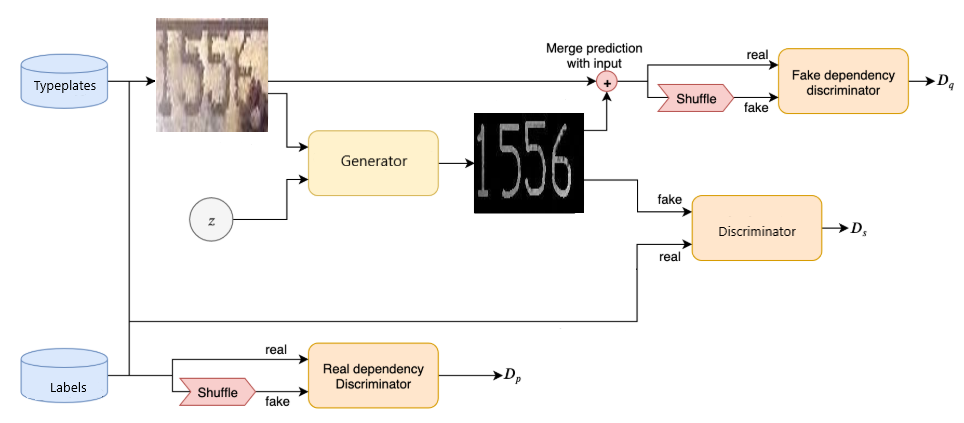
\includegraphics[width=5in]{images/factorgan.PNG}
\caption[Architecture of FactorGAN]{Architecture of FactorGAN. Source: Adapted from \citep{factgit}}
\label{fig:factorgan}
\end{figure}
\subsection{Architecture}
The FactorGAN uses a generator and three discriminators as shown in Figure \ref{fig:factorgan}. The generator generates a clear image of the steel type plate close to the target domain while the discriminator classifies the real and fake image. A real dependency discriminator distinguishes the real steel type plates and its ground truth pairs. A fake dependency discriminator distinguishes the real steel type plates and generated image pairs. 
\begin{figure}
\centering
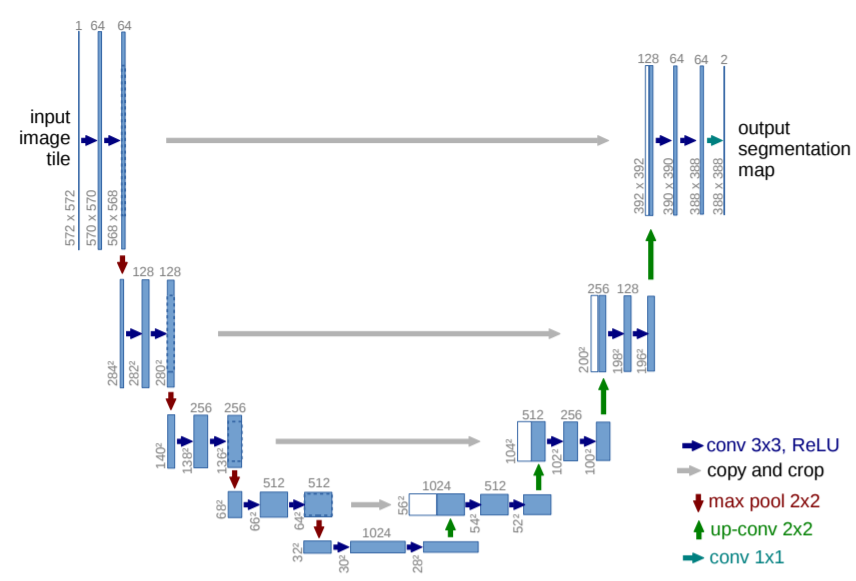
\includegraphics[width=5in]{images/unet.PNG}
\caption[Architecture of U-Net]{Architecture of U-Net. Source: \citep{ronneberger2015u}}\label{fig:unet}
\end{figure}
\subsubsection*{Generator}
The U-Net architecture proposed by \cite{ronneberger2015u} was used for the generator model. U-Net is a fully convolutional neural network that can be composed into three parts: shrinkage, bottleneck and expansion. It consists of conv layers, max pooling, ReLU activation, concatenation layers, up and down sampling as in Figure \ref{fig:unet}. The shrinkage part on the left uses convolution and max pooling operations. The expansion part on the right uses several blocks with upsampling and concatenation \citep{ronneberger2015u}. The full generator architecture is shown in Table \ref{tab:tab5}.
\begin{table}[H]
\centering
\begin{tabular}{|c|c|c|c|} 
\hline
\textbf{Block~} & \textbf{Filters} & \textbf{Filter size~} & \textbf{Stride}  \\ 
\hline
Conv-BN-ReLU    & 32               & 3x3                   & 1                \\ 
\hline
Conv-BN-ReLU    & 32               & 3x3                   & 1                \\ 
\hline
Conv-BN-ReLU    & 64               & 3x3                   & 1                \\ 
\hline
Conv-BN-ReLU    & 64               & 3x3                   & 1                \\ 
\hline
Conv-BN-ReLU    & 128              & 3x3                   & 1                \\ 
\hline
Conv-BN-ReLU    & 128              & 3x3                   & 1                \\ 
\hline
Conv-BN-ReLU    & 256              & 3x3                   & 1                \\ 
\hline
Conv-BN-ReLU    & 256              & 3x3                   & 1                \\ 
\hline
Conv-BN-ReLU    & 256              & 3x3                   & 1                \\ 
\hline
Conv-BN-ReLU    & 256              & 3x3                   & 1                \\ 
\hline
Conv-BN-ReLU    & 128              & 3x3                   & 1                \\ 
\hline
Conv-BN-ReLU    & 128              & 3x3                   & 1                \\ 
\hline
Conv-BN-ReLU    & 64               & 3x3                   & 1                \\ 
\hline
Conv-BN-ReLU    & 64               & 3x3                   & 1                \\ 
\hline
Conv-BN-ReLU    & 32               & 3x3                   & 1                \\ 
\hline
Conv-BN-ReLU    & 32               & 3x3                   & 1                \\ 
\hline
Conv-BN-ReLU    & 32               & 3x3                   & 1                \\ 
\hline
Conv-BN-ReLU    & 32               & 3x3                   & 1                \\ 
\hline
Conv-sigmoid    & 1                & 1x1                   & 1                \\
\hline
\end{tabular}
\caption{Architecture of FactorGAN generator}
\label{tab:tab5}
\end{table}

\subsubsection*{Discriminator}
The architecture of the discriminator is shown in Table \ref{tab:tab6}. It consists of convolution layers with spectral normalization and LReLU activation. All the layers except the fully convolution layer have biases. Spectral normalization normalizes the weight such that the Lipschitz constant for each layer as well as the whole network is one.
\begin{table}[H]
\centering
\begin{tabular}{|c|c|c|c|} 
\hline
\textbf{Block~}        & \textbf{Filters} & \textbf{Filter size~} & \textbf{Stride}  \\ 
\hline
Conv-SN                & 32               & 4x4                   & 2                \\ 
\hline
Block 2 Conv-SN-LReLU~ & 64               & 4x4                   & 2                \\ 
\hline
Block 3 Conv-SN-LReLU~ & 128              & 4x4                   & 2                \\ 
\hline
Block 4 Conv-SN-LReLU~ & 256              & 4x4                   & 2                \\ 
\hline
Block 5 Conv-SN-LReLU~ & 512              & 4x4                   & 2                \\ 
\hline
Block 6 Conv-SN-LReLU~ & 1024             & 4x4                   & 2                \\ 
\hline
Block7 Conv-LReLU      & 1                & 1x1                   & 1                \\
\hline
\end{tabular}
\caption{Architecture of FactorGAN discriminator}
\label{tab:tab6}
\end{table}

\subsection{Objective function}
Let the probability distribution of a dataset is $p_x$ over $x \in \mathbb{R}^d$, discriminator $D_\theta$ and the generator be $G_\phi$ that maps an n dimensional input $z \sim p_z$ to a d dimensional sample $g_\phi(z)$ resulting in the generator distribution $q_x$. Then the loss function \citep{stoller2019training} for standard GAN is given by

\begin{equation*}
arg\underset{\theta}{max}\;\mathbb{E}_{z\sim p_{z}} log D_\theta(G_\phi(z))
\end{equation*}	

To train the GAN with incomplete observation \citep{stoller2019training}, the discriminator D is mapped to a joint density ratio $\frac{p_x(x)}{q_x(x)}$. This joint density ratio is factorized into a product of density ratios.
\begin{align*}
h(\widetilde{D}(x)) = \frac{p_x(x)}{q_x(x)} = \frac{c_P(x)}{c_Q(x)}\prod_{i=1}^{K}\frac{p_x^i(x^i)}{q_x^i(x^i)}\;\;\text{where,}\\c_P(x)= \frac{p_x(x)}{\prod_{i=1}^{K}p_x^i(x^i)}\text{\;\&}\; c_Q(x)= \frac{q_x(x)}{\prod_{i=1}^{K}q_x^i(x^i)}
\end{align*}

For conditional GAN \citep{stoller2019training}, the generator $g_\phi$ that maps a conditional input $x^1$ and a noise to an output $x^2$ resulting in output probability $q_\phi(x^2|x^1)$. In order to eliminate the need for the paired samples, applying the factorization to $x^1$ and $x^2$ with K=2 in the above equation results in 

\begin{equation*}
\frac{p_x(x)}{q_x(x)} = \frac{\frac{p_x(x)}{p_x^1(x^1)p_x^2(x^2)}}{\frac{q_x(x)}{q_x^1(x^1)q_x^2(x^2)}} = \frac{c_P(x)}{c_Q(x)}\frac{p_x^2(x^2)}{q_x^2(x^2)}
\end{equation*}	


From the above equation, \citeauthor{stoller2019training} justified the use of p and q dependency discriminator to model the input-output relationship and a marginal discriminator.
\newline 


\section{Comparison of image-to-image translation GANs under study}
	To summarize, Table \ref{tab:tab7} presents a brief comparison of the above discussed image-to-image translation GANs. The networks describe the complexity of the model with number of generators and discriminators present. Image size denotes the size of input in pixels used in each GAN. Release date is the given publication date for each related article. The method, backbone, normalization and type represent the loss function, architecture, type of normalization and learning approach used for each GAN respectively. 
\begin{table}[H]
\resizebox{\textwidth}{!}{%
\begin{tabular}{|c|c|c|c|}
\hline
                       & \textbf{Pix2pix}           & \textbf{CycleGAN}      & \textbf{FactorGAN}        \\ \hline
\textbf{Method}        & Adversarial loss + L1 loss & Cycle consistency loss & Factorized discriminators \\ \hline
\textbf{Networks} &
  \begin{tabular}[c]{@{}c@{}}1 Generator\\ 1 Discriminator\end{tabular} &
  \begin{tabular}[c]{@{}c@{}}2 Generators \\ 2 Discriminators\end{tabular} &
  \begin{tabular}[c]{@{}c@{}}1 Generator \\ 1 Marginal Discriminator \\ 2 Dependency Discriminators\end{tabular} \\ \hline
\textbf{Image size}    & 600 x 400                  & 300 x 300              & 256 x 256                 \\ \hline
\textbf{Release date}  & 2017 - 2018                & 2017 - 2018            & 2019 - 2020               \\ \hline
\textbf{Normalization} & Batch                      & Instance               & Spectral                  \\ \hline
\textbf{Backbone}      & ResNet                     & ResNet                 & U-Net                      \\ \hline
\textbf{Type} &
  \begin{tabular}[c]{@{}c@{}}Supervised method that\\ requires paired dataset\end{tabular} &
  \begin{tabular}[c]{@{}c@{}}Unsupervised method that\\ requires unpaired dataset\end{tabular} &
  \begin{tabular}[c]{@{}c@{}}Semi-supervised method \\ that handles incomplete\\  data points\end{tabular} \\ \hline
\end{tabular}%
}
\caption{Comparison of image-to-image translation GANs under study}
\label{tab:tab7}
\end{table}
\section{OCR - Text detection}
\cite{baek2019character} proposed Character Region Awareness For Text detection (CRAFT) is the state of the art for scene text detection. We have used the pre-trained model trained using the CRAFT approach in this thesis for text detection.
\newline

	When the problem of text detection is applied to real-world scenarios, it can be seen that the texts in the real world are curved, arbitrary or in an irregular shape. The existing bounding box-based method implemented using the anchor box cannot handle the scenarios where the text is excessively deformed or the text is too large. To improve the text detection in such scenarios, the CRAFT framework was proposed.
\begin{figure}[H]
\centering
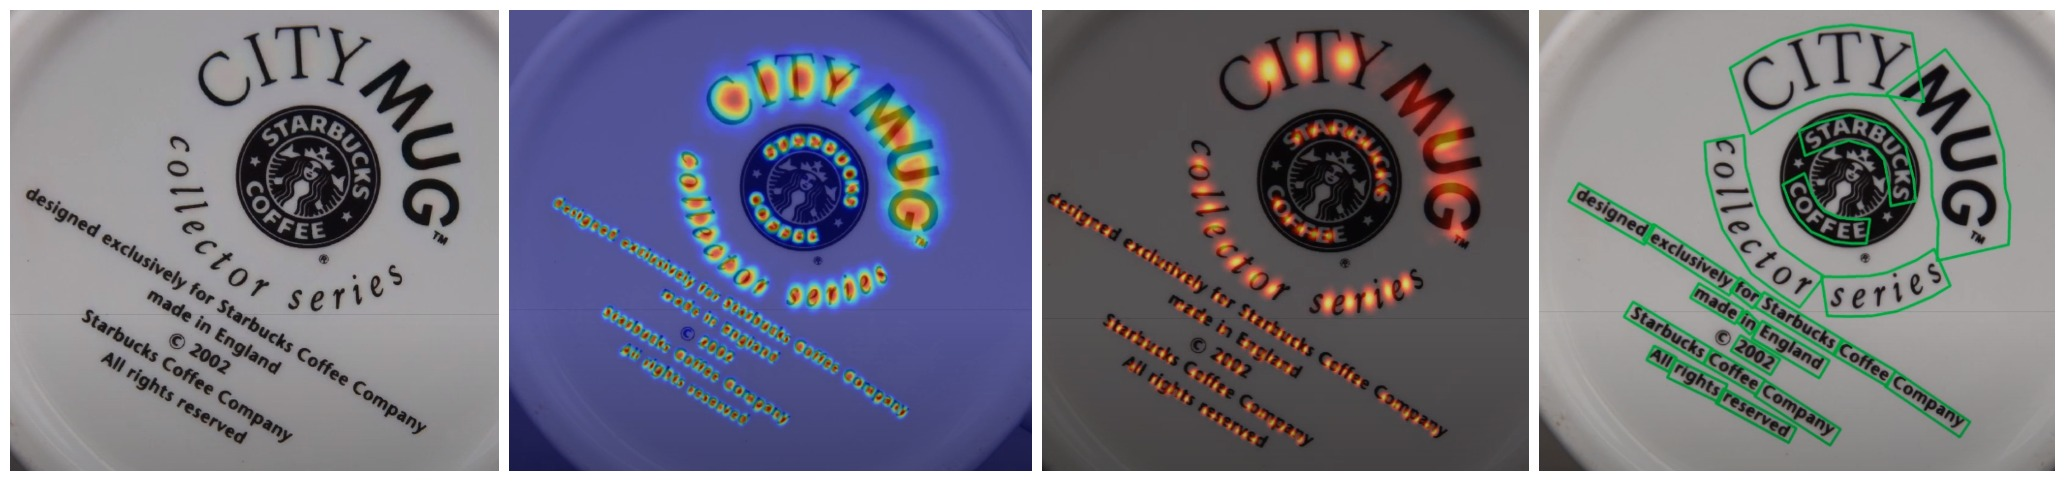
\includegraphics[width=5.5in]{images/craft.jpg}
\caption[The process of CRAFT]{The process of CRAFT: (a) Input image (b) Character region map (c) Affinity score map (d) Text detection output. Source: Adapted from \citep{craft}}
\label{fig:craft}
\end{figure}
The idea of CRAFT is to detect text by exploring each character region and affinity between the characters. It first locates each character in the word using the region score. Then predict whether each character belongs to the same text using the affinity score and concatenate. Thus this model mainly outputs two things:

\begin{enumerate}[(i)]
\item\textbf{Region score} gives the probability of the detected location being a character.
\item\textbf{Affinity score} gives the probability of whether the character at this position needs to be concatenated into a word.
\end{enumerate}


\begin{figure}[H]
\centering
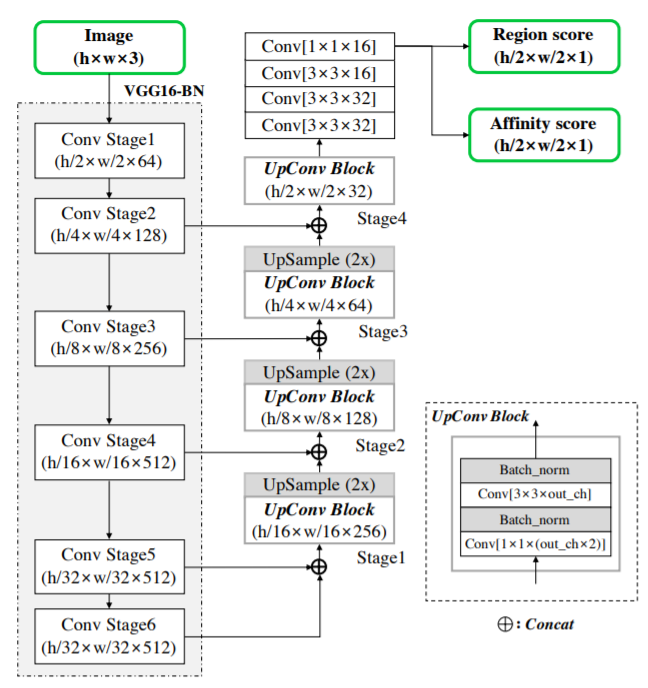
\includegraphics[width=5in]{images/craftarch.png}
\caption[The CRAFT architecture]{The CRAFT architecture. Source: \citep{baek2019character}}
\label{fig:craftarch}
\end{figure} 

The network structure of the CRAFT is shown in Figure \ref{fig:craftarch}. The backbone network is VGG-16, followed by the feature fusion of Feature Pyramid Network. The final output of the model generates a character region prediction (region score) and character association prediction (affinity score). Since the existing datasets for training the text detection models are based on word-level annotations and there is no character level labelling, \citeauthor{baek2019character} used synthetic character dataset for training. The pre-trained model used in this thesis is trained in SynthText \citep{Gupta16}, ICDAR13, ICDAR17 datasets.

\section{OCR - Text recognition}

Several different methods have been proposed in many research works on the scene text recognition. However, each paper that was presented claimed to be the state of the art, there was no fair comparison. \cite{baek2019wrong} in their work presented the fair comparison of different existing methods for scene text recognition. We have utilized their proposed framework for text recognition in this thesis. 

\begin{figure}[H]
\centering
\includegraphics[width=5.5in,scale=1.8]{images/textrec.eps}
\caption[Text recognition framework]{Text recognition framework. Source: \citep{baek2019wrong}}
\label{fig:frame}
\end{figure}

An integrated framework that consists of four stages is proposed for scene text recognition as shown in Figure \ref{fig:frame}. It is as follows:
\begin{enumerate}
\item \textbf{Transformation:}
	The input image in natural scenes comes in arbitrary shapes like curved, vertical, irregular and diverse shapes. Thus the transformation stage uses the \gls{tps}, a variant of \gls{stn} to normalize the input image and transform it into a predefined rectangle.
\item \textbf{Feature extraction:}
	The feature extraction uses CNNs to estimate each character in the receptive field. Their framework has the option to select between ResNet, VGG, and RCNN architecture for feature extraction. We have used ResNet for feature extraction in our OCR engine.
\item \textbf{Sequence modelling:}
	Sequence modelling is used to model the contextual information within the sequence of characters using Bidirectional LSTM (BiLSTM) for robust predictions. 
\item \textbf{Prediction:}
	Attention (Attn) or \gls{ctc} is used to predict a sequence of characters for an input image. We have used Attn as a prediction module for our pre-trained model in this thesis. In the case of CTC, it enables the prediction of a non-fixed number of sequences despite the fixed number of features. The core of CTC seems to be that words can be combined by recognizing letters in each input column and removing repeated letters or blanks. On the other hand, Attn is said to automatically capture the flow of information in the input sequence to predict the output sequence. So, Attn helps the model learn a character-level language modelling that represents class dependencies in the output.
\end{enumerate}

\section{Google Vision OCR}
Google provides an \gls{api} that allows users to integrate many computer vision cloud services such as face detection, logo detection, object detection, text detection, etc to their framework \citep{googleapi}. One such commercial service is the cloud-based OCR that can recognize image files in multiple formats and convert them to text. The API must be enabled first to access the OCR engine and a key for the API needs to be generated. Then the text can be extracted from any number of images that are uploaded. In the work of \citep{compocrs}, they compared different OCR tools available in the market and showed that Google Vision OCR is one of the best tools for optical recognition. We have conducted experiments with the google vision OCR in addition to the proposed OCR to compare and evaluate how good is the proposed OCR engine.


\section{The overall framework}

The proposed framework includes the best generator model from the above-discussed GANs to preprocess the weathered steel type plates. Then the
generated image is passed into OCR engine to extract the text out of it.
\begin{figure}[H]
\centering
\includegraphics[width=5in]{images/overall.eps}
\caption{(a) The overall framework     (b) The proposed OCR }
\label{fig:framework}
\end{figure}
	
	In this thesis, we have studied two different OCR engines 1) Google Vision OCR and 2) The proposed CRAFT based OCR engine with integrated text detection and recognition models. The overall framework is shown in the left of Figure \ref{fig:framework}. 
\newline

	 The proposed OCR engine is shown in the right of Figure
\ref{fig:framework}. It consists of the CRAFT text detection model followed by the text recognition model. The text recognition model uses \gls{tps} for transformation, ResNet as feature extractor, BiLSTM for sequence modelling and Attn for prediction. 


	